\chapter{DESARROLLO DEL PROYECTO}

Se pone a consideraci\'{o}n los siguientes aspectos que se ven convenientes para
describir el proceso desarrollo. para cada objetivo espec\'{i}fico

\begin{itemize}

\item Tarjetas de Historias de Usuario
\item Arquitectura de Componente
\item Modelo de Componente
\item Componente
\item Implementaci\'{o}n de Componente
\item Problema/Soluci\'{o}n de Componente

\end{itemize}

\section{\textquestiondown C\'{o}mo implementar un servicio agregador de noticias?} \label{RSS}

La caracter\'{i}stica de un servicio agregador noticias es realizar notificaciones
via correo electr\'{o}nico respecto a nuevo(s) contenido(s) dentro aplicaci\'{o}n
web sujeto a subscripci\'{o}n, tambi\'{e}n tomando en cuenta que los usuarios 
finales pueden optar por dar de baja la misma. 

\begin{minipage}{1.0\textwidth}
	\centering
	\fbox{
	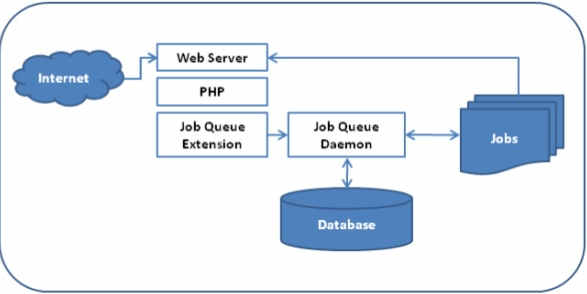
\includegraphics[scale=0.5]{jobQueue}
	}
	\captionof{figure}{Job Queue Architecture}
	\source{fuente:\cite{ossCamp2014}}
	\label{Job Queue Architecture}
\end{minipage}

En la Figura \ref{Job Queue Architecture} se muestra la comunicaci\'{o}n de
componentes que interactuan para ejecutar un proceso en segundo plano 
\footnote{segund plano: Es un programa que se ejecuta sin intervenci\'{o}n del
usuario \cite{background}}, el mismo debe ejecutarse en base fecha liberaci\'{o}n definida en un
podcast al momento del registro.   

\subsection{Tarjetas de Historias de Usuario}

Las Historias de Usuario se elaboran en base a deseos de Carrera LAEL y
gestionado por un Coordinador designado como responsable del proyecto 
adscripci\'{o}n, el mismo que sugirio cambios de funcionalidades en el
transcurso del tiempo.

% add history card 03
\begin{minipage}[b]{\hsize}\centering
\begin{tabular}{|l|l|l|}
\hline
 & \textbf{Tarjeta Historia de Usuario} &  \\ \hline
ID Historia: 03 & \begin{tabular}[c]{@{}l@{}}Nombre: Suscripción a un\\ Podcast de un Aprendiz\\ Autorregulado.\end{tabular} & Fecha: 22/04/2014 \\ \hline
\multicolumn{3}{|l|}{Rol: Aprendiz Autorregulado} \\ \hline
\begin{tabular}[c]{@{}l@{}}Modificación de Historia\\ Numero: 05\end{tabular} & \begin{tabular}[c]{@{}l@{}}Iteración Asignada: 7,8,\\ 9, 11\end{tabular} & Prioridad en Negocio: Medio \\ \hline
Tiempo Estimado Inicial: 20 & Riesgo en Desarrollo: & Tipo de Historia: Funcional \\ \hline
\multicolumn{3}{|l|}{\begin{tabular}[c]{@{}l@{}}Descripción:\\ \\ Yo como usuario Aprendiz Autorregulado deseo suscribirme a un Podcast de un determinado\\ idioma, tal que solo pinchar en el botón de suscripción (para esto ya no necesito ingresar mi\\ correo electrónico).\end{tabular}} \\ \hline
\multicolumn{3}{|l|}{\begin{tabular}[c]{@{}l@{}}Pre Condición:	\\ \\ Usuario Autentificado. \\ Contenido publicado. \\ Servidor SMTP configurado.\end{tabular}} \\ \hline
\multicolumn{3}{|l|}{\begin{tabular}[c]{@{}l@{}}Post Condición:\\ \\ Recibir mensajes en mi bandeja de entrada de mi cuenta de correo.\end{tabular}} \\ \hline
\multicolumn{3}{|l|}{\begin{tabular}[c]{@{}l@{}}Observaciones:\\ \\ La suscripción del usuario Aprendiz Autorregulado le permite acceder solo a un  producto,\\ sin permitirle dejar comentarios o interactuar de otra manera en la plataforma.\end{tabular}} \\ \hline
\begin{tabular}[c]{@{}l@{}}.....................................................\\ Msc. Lic. Vladimir Costas Juaregui\\ PROJECT MANAGER\end{tabular} & \begin{tabular}[c]{@{}l@{}}..........................................\\ Lic. Manuel Camacho Arce\\ PRODUCT OWNER\end{tabular} & \begin{tabular}[c]{@{}l@{}}.........................................\\ Juan Omar Huanca Balboa\\ SCRUM MASTER\end{tabular} \\ \hline
\end{tabular}
\captionof{table}{Tarjeta Historia de Usuario 03}
\source{fuente: (Elaboraci\'{o}n Propia)}
\label{Tarjeta Historia de Usuario 03}
\end{minipage}

% add user history card 57
\begin{minipage}[b]{\hsize}\centering
\begin{tabular}{|l|l|l|}
\hline
 & \textbf{Tarjeta Historia de Usuario} &  \\ \hline
ID Historia: 57 & \begin{tabular}[c]{@{}l@{}}Nombre: Personalización\\  Subscripción \\ Sub Categorias.\end{tabular} & Fecha: 22/04/2014 \\ \hline
\multicolumn{3}{|l|}{Rol: Aprendiz Autorregulado/ Tutor/ Coordinador/ Administrador} \\ \hline
\begin{tabular}[c]{@{}l@{}}Modificación de Historia\\ Numero:\end{tabular} & Iteración Asignada: 11 & Prioridad en Negocio: Medio \\ \hline
Tiempo Estimado Inicial: 20 & Riesgo en Desarrollo: & Tipo de Historia: Funcional \\ \hline
\multicolumn{3}{|l|}{\begin{tabular}[c]{@{}l@{}}Descripción:\\ \\ Yo como usuario Aprendiz Autorregulado, Tutor, Coordinador, Administrador\\ deseo poder personalizar mi subscripción tal que me beneficie en poder escoger mis \\ intereses de subcategorias.\end{tabular}} \\ \hline
\multicolumn{3}{|l|}{\begin{tabular}[c]{@{}l@{}}Pre Condición:	\\ \\ Usuario Autentificado.\end{tabular}} \\ \hline
\multicolumn{3}{|l|}{\begin{tabular}[c]{@{}l@{}}Post Condición:\\ \\ Agregar a mis intereses la sub categoria.\end{tabular}} \\ \hline
\multicolumn{3}{|l|}{\begin{tabular}[c]{@{}l@{}}Observaciones:\\ \\ El usuario al momento de regitrarse a un contenido, estara subscrito a\\ todo el programa de aprendizaje.\end{tabular}} \\ \hline
\begin{tabular}[c]{@{}l@{}}.....................................................\\ Msc. Lic. Vladimir Costas Juaregui\\ PROJECT MANAGER\end{tabular} & \begin{tabular}[c]{@{}l@{}}..........................................\\ Lic. Manuel Camacho Arce\\ PRODUCT OWNER\end{tabular} & \begin{tabular}[c]{@{}l@{}}.........................................\\ Juan Omar Huanca Balboa\\ SCRUM MASTER\end{tabular} \\ \hline
\end{tabular}
\captionof{table}{Tarjeta Historia de Usuario 57}
\source{fuente: (Elaboraci\'{o}n Propia)}
\label{Tarjeta Historia de Usuario 57}
\end{minipage}

% add user history card 56
\begin{minipage}[b]{\hsize}\centering
\begin{tabular}{|l|l|l|}
\hline
 & \textbf{Tarjeta Historia de Usuario} &  \\ \hline
ID Historia: 56 & \begin{tabular}[c]{@{}l@{}}Nombre: Liberación \\ de contenidos\end{tabular} & Fecha: 03/05/2015 \\ \hline
\multicolumn{3}{|l|}{Rol: Tutor} \\ \hline
\begin{tabular}[c]{@{}l@{}}Modificación de Historia\\ Numero:\end{tabular} & Iteración Asignada: 10 & Prioridad en Negocio: Medio \\ \hline
Tiempo Estimado Inicial: 35 & Riesgo en Desarrollo: & Tipo de Historia: Funcional \\ \hline
\multicolumn{3}{|l|}{\begin{tabular}[c]{@{}l@{}}Descripción:\\ \\ Yo como usuario Tutor deseo definir la liberación de mis Episodios definidos anteriormente\\ en el registro tal que me beneficie una publicación cronologica respecto a un Programa\\ de Aprendizaje.\end{tabular}} \\ \hline
\multicolumn{3}{|l|}{\begin{tabular}[c]{@{}l@{}}Pre Condición:	\\ \\ Usuario Autentificado.\end{tabular}} \\ \hline
\multicolumn{3}{|l|}{Post Condición:} \\ \hline
\multicolumn{3}{|l|}{\begin{tabular}[c]{@{}l@{}}Observaciones:\\ \\ La liberación de los contenidos deberia estar bajo un cronograma de liberación secuencial.\end{tabular}} \\ \hline
\begin{tabular}[c]{@{}l@{}}.....................................................\\ Msc. Lic. Vladimir Costas Juaregui\\ PROJECT MANAGER\end{tabular} & \begin{tabular}[c]{@{}l@{}}..........................................\\ Lic. Manuel Camacho Arce\\ PRODUCT OWNER\end{tabular} & \begin{tabular}[c]{@{}l@{}}.........................................\\ Juan Omar Huanca Balboa\\ SCRUM MASTER\end{tabular} \\ \hline
\end{tabular}
\captionof{table}{Tarjeta Historia de Usuario 56}
\source{fuente: (Elaboraci\'{o}n Propia)}
\label{Tarjeta Historia de Usuario 56}
\end{minipage}

% add user history card 58
\begin{minipage}[b]{\hsize}\centering
\begin{tabular}{|l|l|l|}
\hline
 & \textbf{Tarjeta Historia de Usuario} &  \\ \hline
ID Historia: 58 & \begin{tabular}[c]{@{}l@{}}Nombre: Darse de baja \\ subscripción podcast Aprendiz\\ Autorregulado.\end{tabular} & Fecha: 19/05/2015 \\ \hline
\multicolumn{3}{|l|}{Rol: Aprendiz Autorregulado} \\ \hline
\begin{tabular}[c]{@{}l@{}}Modificación de Historia\\ Numero: 04\end{tabular} & Iteración Asignada: 11 & Prioridad en Negocio: Bajo \\ \hline
Tiempo Estimado Inicial: 15 & Riesgo en Desarrollo: & Tipo de Historia: Funcional \\ \hline
\multicolumn{3}{|l|}{\begin{tabular}[c]{@{}l@{}}Descripción:\\ \\ Yo como usuario Aprendiz Autorregulado deseo dar de baja mi suscripción de un determinado \\ Podcast de algún canal de noticias tal que me beneficie de no recibir más notificaciones.\\ \\ Para esto necesito pinchar en un enlace con la etiqueta Dar de baja dentro del cuerpo\\ de un mensaje.\end{tabular}} \\ \hline
\multicolumn{3}{|l|}{\begin{tabular}[c]{@{}l@{}}Pre Condición:\\ \\ Usuario Autentificado. \\ Usuario Suscrito\end{tabular}} \\ \hline
\multicolumn{3}{|l|}{\begin{tabular}[c]{@{}l@{}}Post Condición:\\ \\ Dejar de recibir notificaciones a mi bandeja de entrada.\end{tabular}} \\ \hline
\multicolumn{3}{|l|}{\begin{tabular}[c]{@{}l@{}}Como Probarlo:\\ \\ Pinchar en el enlace que aparece en cada mensaje de noticias y pinchar.\end{tabular}} \\ \hline
\begin{tabular}[c]{@{}l@{}}.....................................................\\ Msc. Lic. Vladimir Costas Juaregui\\ PROJECT MANAGER\end{tabular} & \begin{tabular}[c]{@{}l@{}}..........................................\\ Lic. Manuel Camacho Arce\\ PRODUCT OWNER\end{tabular} & \begin{tabular}[c]{@{}l@{}}.........................................\\ Juan Omar Huanca Balboa\\ SCRUM MASTER\end{tabular} \\ \hline
\end{tabular}
\captionof{table}{Tarjeta Historia de Usuario 58}
\source{fuente: (Elaboraci\'{o}n Propia)}
\label{Tarjeta Historia de Usuario 58}
\end{minipage}

\subsection{Arquitectura de Componente}

En la Figura \ref{fig:Diagrama Caso de Uso Subscripci\'{o}n} se identifica los 
diferentes procesos Actores como ser: Coordinador, Administrador, Tutor, 
Autorregulado que tienen eventos dentro el sistema mediante procesos descritas
en un lenguaje natural en Cuadro \ref{Tarjeta Historia de Usuario 03}, Cuadro
\ref{Tarjeta Historia de Usuario 58}

\begin{minipage}{1.0\textwidth}
	\centering
	\fbox{
		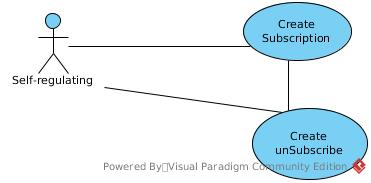
\includegraphics[scale=0.6]{caseUseSubscription}
	}
	\captionof{figure}{Diagrama Caso de Uso Subscripci\'{o}n}
	\source{fuente: (Elaboraci\'{o}n Propia)}
	\label{fig:Diagrama Caso de Uso Subscripci\'{o}n}
\end{minipage}

En la Figura \ref{fig:Diagrama Clases Subscripci\'{o}n} se identifica la
representaci\'{o}n de datos por cada Clase, attibutos y composici\'{o}n.

\begin{minipage}{1.0\textwidth}
	\centering
	\fbox{
		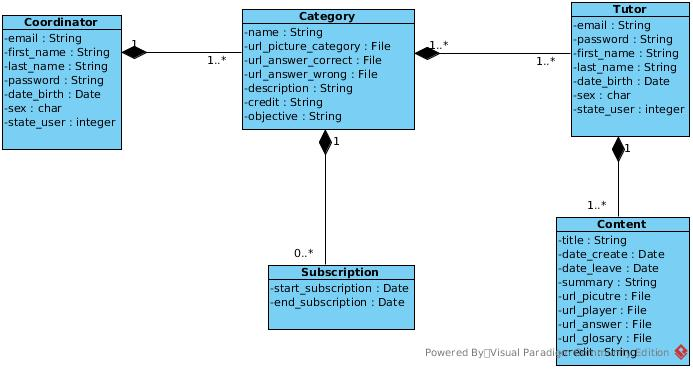
\includegraphics[scale=0.6]{classSubscription}
	}
	\captionof{figure}{Diagrama Clases Subscripci\'{o}n}
	\source{fuente: (Elaboraci\'{o}n Propia)}
	\label{fig:Diagrama Clases Subscripci\'{o}n}
\end{minipage}

En la Figura \ref{fig:Diagrama Secuencia Subscripci\'{o}n} se realiza la
representaci\'{o}n de subscripci\'{o}n en forma din\'{a}mica. Adem\'{a}s se 
realiza la representaci\'{o}n sobre la acci\'{o}n dar de baja por programa
aprendizaje (category), brindando un historial en el tiempo sobre los registros. 

\begin{minipage}{1.0\textwidth}
\centering
\fbox{
	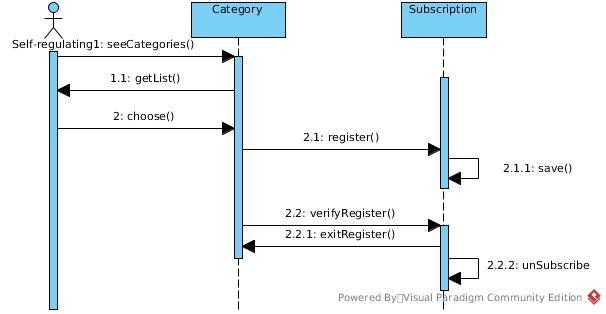
\includegraphics[scale=0.7]{sequenceSubscription}
}
\captionof{figure}{Diagrama Secuencia Subscripci\'{o}n}
\source{fuente: (Elaboraci\'{o}n Propia)}
\label{fig:Diagrama Secuencia Subscripci\'{o}n}
\end{minipage}

\subsection{Modelo de Componente}

En la Figura \ref{fig:Modelo Subscripci\'{o}n Modelo de Datos} se define el 
modelo parcial base de datos respecto a personalizaci\'{o}n en subscripci\'{o}n
de un programa de aprendizaje orientado a un rol autentificado. 

\begin{minipage}{1.0\textwidth}
	\centering
	\fbox{
		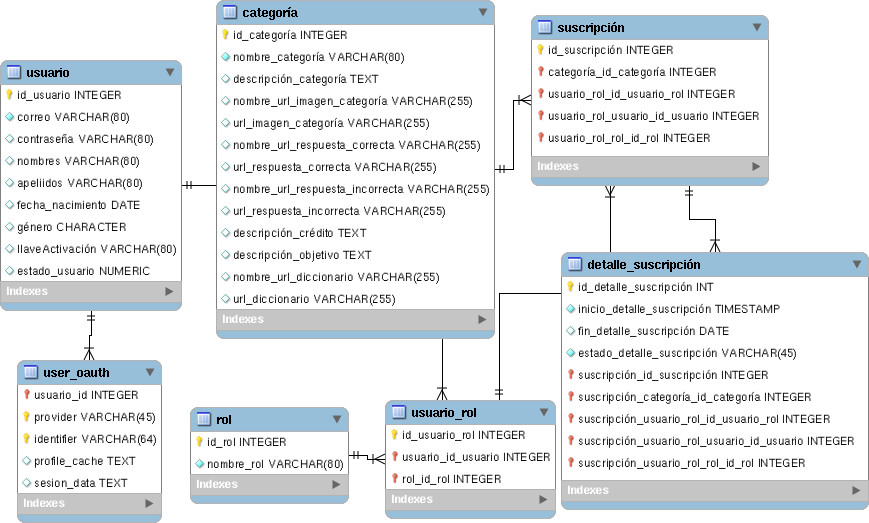
\includegraphics[scale=0.5]{modelSubscription}
	}
	\captionof{figure}{Modelo Subscripci\'{o}n Modelo de Datos}
	\source{fuente: (Elaboraci\'{o}n Propia)}
	\label{fig:Modelo Subscripci\'{o}n Modelo de Datos}
\end{minipage}

Se define subscripci\'{o}n por programa aprendizaje (category), este debe ser
sujeto a notificaci\'{o}n, tomando en cuenta que dentro del sistema un usuario
puede llegar a tener m\'{a}s de un rol asignado. Adem\'{a}s se considera 
mantener una bit\'{a}cora \footnote{bit\'{a}cora: Mecanismo persistencia de 
actividades en el tiempo (Elaboraci\'{o}n Propia)} (detail\textunderscore 
subscription) de acciones de subscripci\'{o}n y dar de baja la 
subscripci\'{o}n realizadas.

\subsection{Componente}

En la Figura \ref{fig:Ventana emergente subscripci\'{o}n} se opta por 
subscripci\'{o}n por programa de aprendizaje (sub-categor\'{i}a), el
usuario debe autentificarse para poder subscribirse.

Se brinda dos opciones para la subscripci\'{o}n como ser: Primera Opci\'{o}n
Manual, la misma permite ingresar solo una direcci\'{o}n de correo sujeto a verificaci\'{o}n
Segunda Opci\'{o}n Red Social, Google, Facebook, Twitter. 

\begin{minipage}{1.0\textwidth}
	\centering
	\fbox{
		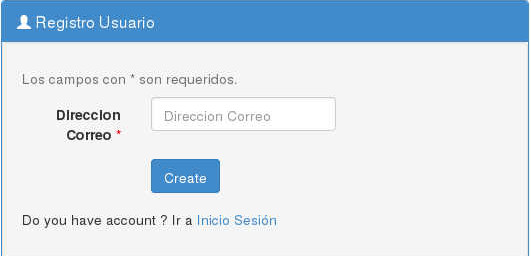
\includegraphics[scale=0.6]{modalSubscribe}
	}
	\captionof{figure}{Ventana emergente subscripci\'{o}n}
	\source{fuente: (Elaboraci\'{o}n Propia)}
	\label{fig:Ventana emergente subscripci\'{o}n}
\end{minipage}

En la Figura \ref{fig:Formulario de Autentificaci\'{o}n} una opci\'{o}n emergente
luego de pinchar sobre opci\'{o}n Inicio Sesi\'{o}n. Se Ingresa a Sistema con
los siguientes campos: Nombre Usuario, Contrase\~{n}a.

\begin{minipage}{1.0\textwidth}
	\centering
	\fbox{
		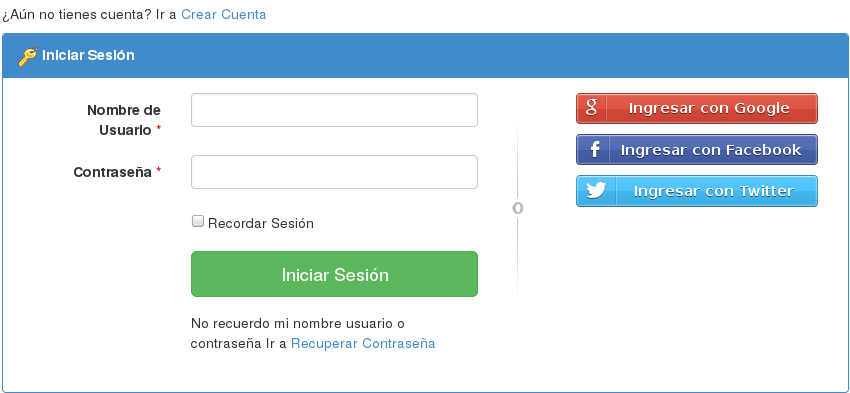
\includegraphics[scale=0.6]{login}
	}
	\captionof{figure}{Formulario de Autentificaci\'{o}n}
	\source{fuente: (Elaboraci\'{o}n Propia)}
	\label{fig:Formulario de Autentificaci\'{o}n}
\end{minipage}

En la Figura \ref{fig:Facebook OAuth Autenticatition} se facilita el Diagrama 
Secuencia en uso de un servicio externo, para facilitar un acceso, partiendo
de una cuenta v\'{a}lida dentro los usuarios en Facebook.

\begin{minipage}{1.0\textwidth}
	\centering
	\fbox{
		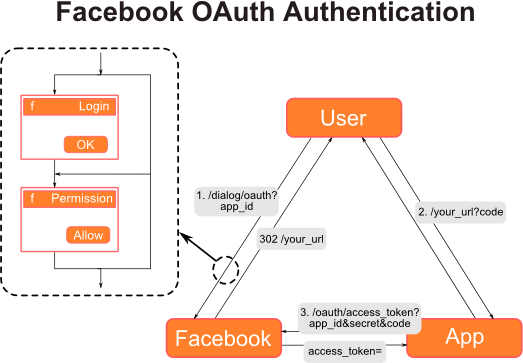
\includegraphics[scale=0.4]{oauthFacebook}
	}
	\captionof{figure}{Facebook OAuth Autenticatition}
	\source{fuente: \cite{oauthFacebook}}
	\label{fig:Facebook OAuth Autenticatition}
\end{minipage}

En la Figura \ref{Aplicaciones de servidor web} se facilita el Diagrama Secuencia
en uso de un servicio externo, para facilitar un acceso, partiendo de una cuenta
v\'{a}lida dentro los usuarios en Google.

\begin{minipage}{1.0\textwidth}
	\centering
	\fbox{
		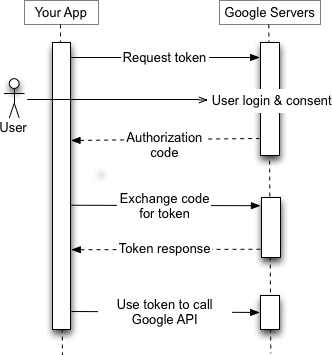
\includegraphics[scale=0.6]{oauth20Google}
	}
	\captionof{figure}{Aplicaciones de servidor web}
	\source{fuente: \cite{oauthGoogle}}
	\label{Aplicaciones de servidor web}
\end{minipage}

En la Figura \ref{Aplicaci\'{o}n de solo autentificaci\'{o}n} se facilita el 
Diagrama Secuencia en uso de un servicio externo, para facilitar un acceso,
partiendo de una cuenta v\'{a}lida dentro los usuarios en Twitter.

\begin{minipage}{1.0\textwidth}
	\centering
	\fbox{
		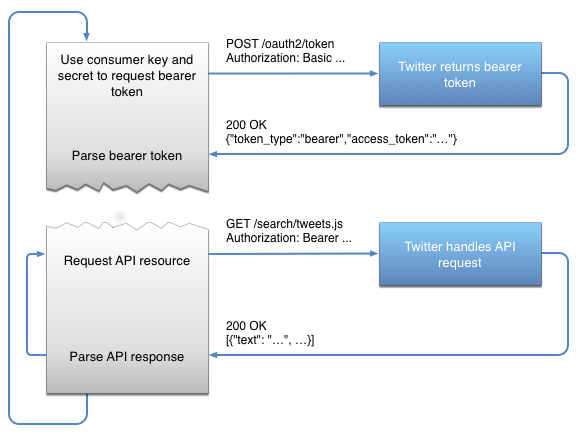
\includegraphics[scale=0.5]{oauth10Twitter}
	}
	\captionof{figure}{Aplicaci\'{o}n de solo autentificaci\'{o}n}
	\source{fuente: \cite{oauthTwitter}}
	\label{Aplicaci\'{o}n de solo autentificaci\'{o}n}
\end{minipage}
	
\subsection{Implementaci\'{o}n de Componente}

\begin{itemize}

\item \textbf{Implementaci\'{o}n en el Servidor} Se define el siguiente Segmento
C\'{o}digo donde se personaliza la subscripci\'{o}n por programa de aprendizaje.
El cual permite poder visualizar programas de aprendizaje habilitados sujetos a
subscripci\'{o}n.

\begin{lstlisting}[language = PHP]
public function actionCustomRss($idCategory) {
ob_end_clean();
header('Content-type: text/xml; charset=utf-8');
// turn off layout
$this->layout = false;
// add custom criteria
$criteria = new CDbCriteria;
$criteria->addCondition('t.category_id_category=:Column1');
$criteria->addCondition('t.category_id_category in (select 
i.category_id_category from interest as i) and t.content_status=
'.Yii::app()->params['stateContentAvailable']);
$criteria->select = 't.title,t.summary,t.date_leave';
$criteria->params = array(':Column1' => $idCategory);
$data = Content::model()->findAll($criteria);
// redirect view
$this->renderPartial('_viewItemChannel', array('data' => $data));
}
\end{lstlisting}

En la linea 2 se tiene por funcionalidad de: Limpiar el b\'{u}ffer de
salida y deshabilitar el uso del b\'{u}ffer de salida.

En la linea 3 es agrega la cabecera de un documento XML y su respectiva
codificaci\'{o}n en UTF-8 \footnote{UTF-8: El est\'{a}ndar Unicode cubre todos
los caracteres, signos de puntuaci\'{o}n y s\'{i}mbolos en el mundo. Unicode 
procesamiento, almacenamiento y transporte de texto, independiente de la 
plataforma y lenguaje \cite{utf8}}

\item \textbf{Implementaci\'{o}n en el Servidor} Se define por medio de contrab
un shell sobre una distribuci\'{o}n linux especificar la funci\'{o}n asincrona
permite ejecutar script ejecuci\'{o}n de liberaci\'{o}n de podcast el cual 
realiza la comparaci\'{o}n de la fecha actual con la fecha de liberaci\'{o}n.

\begin{lstlisting}[language = PHP]
public function run($args) {	
$jobs = $this->getJobs();
foreach ($jobs as $job) {
	...
    // set field available
    $job->content_status = Yii::app()->params['stateContentAvailable'];
    // save data
    $job->save();
    $this->sendMailSubscribed($job->category_id_category, 
    $job->user_id_user, $job->title, $job->summary);
}
}
\end{lstlisting}

\end{itemize}

\subsection{Problema/Soluci\'{o}n de Componente}

Se consideran las siguientes dificultades que surgieron para la implementaci\'{o}n
para el Servicio Agregador de Noticias.

\begin{itemize}

\item Generaci\'{o}n \'{u}nica de modal \footnote{modal: Una ventana modal es, 
por tanto, normalmente una ventana secundaria. El usuario tiene que interactuar
con \'{e}l antes de que el control se pueda devolver a la solicitud principal
\cite{modal}} respecto a Programa Aprendizaje (sub-categor\'{i}a)
\item Env\'{i}o de mensaje de notificaci\'{o}n de liberaci\'{o}n contenido tarea
en segundo plano. 

\end{itemize}

En la generaci\'{o}n de varias programas de aprendizaje sobre una lista con acceso a
una ventana modal sujeto subscripci\'{o}n, este identificador anteriormente
ten\'{i}a asignado siempre el mismo identificador del \'{u}ltimo programa.

\begin{enumerate}

\item \textbf{Generar \'{U}nico identificador por Modal - Implementaci\'{o}n en
el Cliente}

Se define como mecanismo de soluci\'{o}n para generar un identidicador como ser:
Categor\'{i}a: Frances, Programa Aprendizaje: Frances B\'{a}sico. Categor\'{i}a:
Ingl\'{e}s, Programa Aprendizaje: Ingl\'{e}s B\'{a}sico. Categor\'{i}a: Quechua,
Programa Aprendizaje: Quechua B\'{a}sico, Quechua Psicosocial. Categor\'{i}a: Quechua,
Programa Aprendizaje: Fon\'{e}tica Quechua

\begin{lstlisting}[]
<?php $this->beginWidget(
        'booster.widgets.TbModal', array(
    'id' => 'myModal' . $category_id,
));?>
<div class="modal-body">
    <div class="panel-body">
        <?php $this->renderPartial('//site/createRegisterSuscribe', 
        array('model_user' => $model_user)); ?>
    </div>
</div>
<?php $this->endWidget(); ?>
\end{lstlisting}

Se tubo problemas al momento de enviar la notificaci\'{o}n a las cuentas de correo
que se encuentran subscritos a un programa de aprendizaje, debido que el mensaje de 
correo contiene etiquetas propias de HTML \footnote{HTML: Es el conjunto de 
s\'{i}mbolos de marcado o c\'{o}digos insertados en un archivo destinado a la
visualizaci\'{o}n de una p\'{a}gina Web Mundial. \cite{html}} 

\item \textbf{Envio Mensajes - Implementaci\'{o}n en el Servidor}

Se define Segmento C\'{o}digo como la implementaci\'{o}n de envio de mail con la 
caracter\'{i}stica de que muestra el mensaje de correo sin p\'{a}gina maestra.

\begin{lstlisting}[language = PHP]
private function sendMailSubscribed($idCategory, $idUser,
$title, $summary) {
$userRols = Category::model()->getRecentUserSubscribe($idCategory);
foreach ($userRols->categoryUserRol as $userRol) {
if ($idUser != $userRol->user_id_user) {
// set properties
$subject = Yii::app()->params['setSubjectContentRelease'];
$body = Yii::app()->params['setBodyContentRelease'] . $title . $summary
. Yii::app()->params['setBodyBelowContentRelease'] . 
Yii::app()->params['adminEmail'] . 
Yii::app()->params['setBodyBottomContentRelease'];
$to = $userRol->userIdUser->email;
// send mail
$mail = new YiiMailer();
//use "cron" view from views/mail
$mail->setBody($body);
$mail->setData(array('message' => $subject, 'name' => get_class($this),
'description' => 'Cron job', 'mailer' => $mail));
//render HTML mail, layout is set from config file or with 
//$mail->setLayout('layoutName')
$mail->render();
//set properties as usually with PHPMailer
$mail->From = Yii::app()->params['adminEmail'];
$mail->FromName = Yii::app()->params['fromNameConsole'];
$mail->Subject = $subject;
$mail->AddAddress($to);
...
}
}
}
\end{lstlisting}

\end{enumerate}

\section{\textquestiondown Como Implementar Mecanismos de Transcripci\'{o}n?}

Se desea poder integrar el reproductor de un Podcast con su propia conversaci\'{o}n
de tal forma se tenga un efecto de mayor compensi\'{o}n auditiva y visual.
Tambi\'{e}n se desea poder generar definici\'{o}n de palabras referentes a contenido
Podcast de forma textual.
 
\subsection{Tarjetas de Historias de Usuario}

Las Tarjetas de Historias de Usuario son aquellas que representan los deseos de la
Unidad Patrocinadora representados por su Coordinador en lenguaje natural, para 
definir la funcionalidad de parte del sistema.

% add user history card 59
\begin{minipage}[b]{\hsize}\centering
\begin{tabular}{|l|l|l|}
\hline
 & \textbf{Tarjeta Historia de Usuario} &  \\ \hline
ID Historia: 59 & \begin{tabular}[c]{@{}l@{}}Nombre: Gestionar\\ Karaoke podcast\end{tabular} & Fecha: 09/05/2015 \\ \hline
\multicolumn{3}{|l|}{Rol: Tutor} \\ \hline
\begin{tabular}[c]{@{}l@{}}Modificación de Historia\\ Numero:\end{tabular} & Iteración Asignada: 14 & Prioridad en Negocio: Medio \\ \hline
Tiempo Estimado Inicial: 35 & Riesgo en Desarrollo: & Tipo de Historia: Funcional \\ \hline
\multicolumn{3}{|l|}{\begin{tabular}[c]{@{}l@{}}Descripción:\\ \\ Yo como usuario Tutor deseo tener un karaoke tal que me beneficie poder relacionar\\ el reproductor con la conversación del podcast.\\ \\ Para esto necesito: Tipo Traducción, Frase, Lenguage (Destino), Significado,\\ Tiempo Inicio, Tiempo Fin.\end{tabular}} \\ \hline
\multicolumn{3}{|l|}{\begin{tabular}[c]{@{}l@{}}Pre Condición:	\\ \\ Usuario Autentificado.\end{tabular}} \\ \hline
\multicolumn{3}{|l|}{Post Condición:} \\ \hline
\multicolumn{3}{|l|}{\begin{tabular}[c]{@{}l@{}}Como Probarlo:\\ \\ Se tiene que pinchar sobre botón play reproductor\\
pinchar dos veces sobre el boton Mostrar/Ocultar\\ Transcripción, para poder apreciar la transcripción además de una \\
 traducción a un lenguaje destino.\end{tabular}} \\ \hline
\begin{tabular}[c]{@{}l@{}}.....................................................\\ Msc. Lic. Vladimir Costas Juaregui\\ PROJECT MANAGER\end{tabular} & \begin{tabular}[c]{@{}l@{}}..........................................\\ Lic. Manuel Camacho Arce\\ PRODUCT OWNER\end{tabular} & \begin{tabular}[c]{@{}l@{}}.........................................\\ Juan Omar Huanca Balboa\\ SCRUM MASTER\end{tabular} \\ \hline
\end{tabular}
\captionof{table}{Tarjeta Historia de Usuario 59}
\source{fuente: (Elaboraci\'{o}n Propia)}
\label{Tarjeta Historia de Usuario 59}
\end{minipage}

% add user history card 60
\begin{minipage}[b]{\hsize}\centering
\begin{tabular}{|l|l|l|}
\hline
 & \textbf{Tarjeta Historia de Usuario} &  \\ \hline
ID Historia: 60 & \begin{tabular}[c]{@{}l@{}}Nombre: Gestionar\\ Glosario audio podcast\end{tabular} & Fecha: 19/05/2015 \\ \hline
\multicolumn{3}{|l|}{Rol: Tutor} \\ \hline
\begin{tabular}[c]{@{}l@{}}Modificación de Historia\\ Numero: 04\end{tabular} & Iteración Asignada: 14 & Prioridad en Negocio: Medio \\ \hline
Tiempo Estimado Inicial: 30 & Riesgo en Desarrollo: & Tipo de Historia: Funcional \\ \hline
\multicolumn{3}{|l|}{\begin{tabular}[c]{@{}l@{}}Descripción:\\ \\ Yo como usuario Tutor deseo gestionar un glosario tal que me beneficie poder definir términos \\ por cada Episodio.\\ \\ Para esto necesito: Tipo Traducción, Frase, Lenguage (Destino), Significado.\end{tabular}} \\ \hline
\multicolumn{3}{|l|}{\begin{tabular}[c]{@{}l@{}}Pre Condición:\\ \\ Usuario Autentificado.\end{tabular}} \\ \hline
\multicolumn{3}{|l|}{\begin{tabular}[c]{@{}l@{}}Como Probarlo: \\ \\ Se tiene que situar sobre detalle Podcast, para luego pinchar sobre la segunda\\ opción Definición Glosario dentro del Tab de opciones.\end{tabular}} \\ \hline
\multicolumn{3}{|l|}{\begin{tabular}[c]{@{}l@{}}Observaciones:\\ \\ Se realizara al gestión para podcast de tipo audio.\end{tabular}} \\ \hline
\begin{tabular}[c]{@{}l@{}}.....................................................\\ Msc. Lic. Vladimir Costas Juaregui\\ PROJECT MANAGER\end{tabular} & \begin{tabular}[c]{@{}l@{}}..........................................\\ Lic. Manuel Camacho Arce\\ PRODUCT OWNER\end{tabular} & \begin{tabular}[c]{@{}l@{}}.........................................\\ Juan Omar Huanca Balboa\\ SCRUM MASTER\end{tabular} \\ \hline
\end{tabular}
\captionof{table}{Tarjeta Historia de Usuario 60}
\source{fuente: (Elaboraci\'{o}n Propia)}
\label{Tarjeta Historia de Usuario 60}
\end{minipage}

\subsection{Arquitectura de Componente}

En la Figura \ref{fig:Diagrama Caso de Uso Traducci\'{o}n} se realiza la 
representaci\'{o}n de funcionalidad especificada Procesos, Actores definida en
los Cuadros  \ref{Tarjeta Historia de Usuario 59}, Cuadro \ref{Tarjeta Historia
de Usuario 60}

\begin{minipage}{1.0\textwidth}
	\centering
	\fbox{
		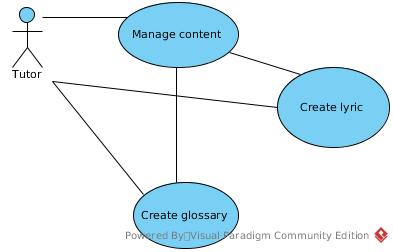
\includegraphics[scale=0.7]{caseUseTranslation}
	}
	\captionof{figure}{Diagrama Caso de Uso Traducci\'{o}n}
	\source{fuente: (Elaboraci\'{o}n Propia)}
	\label{fig:Diagrama Caso de Uso Traducci\'{o}n}
\end{minipage}

En la Figura \ref{fig:Diagrama Clases Traducci\'{o}n} se realiza la
representaci\'{o}n de Datos por medio de Clases: Tutor, Content, Lyric, 
Glossary.

\begin{minipage}{1.0\textwidth}
	\centering
	\fbox{
		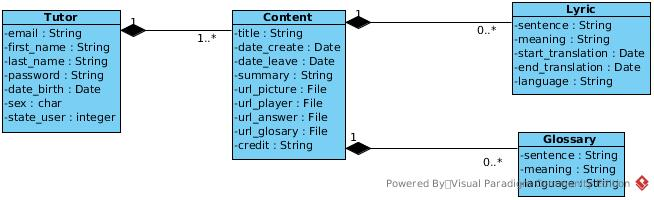
\includegraphics[scale=0.7]{classTranslation}
	}
	\captionof{figure}{Diagrama Clases Traducci\'{o}n}
	\source{fuente: (Elaboraci\'{o}n Propia)}
	\label{fig:Diagrama Clases Traducci\'{o}n}
\end{minipage}

En la Figura \ref{fig:Diagrama Secuencia Traducci\'{o}n} se realiza la 
interacci\'{o}n de Clases y Actor.

\begin{minipage}{1.0\textwidth}
	\centering
	\fbox{
		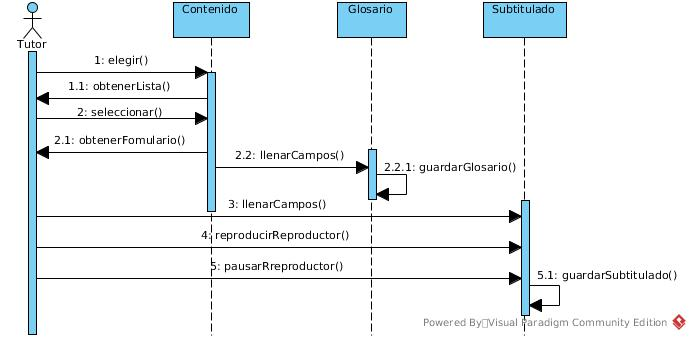
\includegraphics[scale=0.6]{sequenceTranslation}
	}
	\captionof{figure}{Diagrama Secuencia Traducci\'{o}n}
	\source{fuente: (Elaboraci\'{o}n Propia)}
	\label{fig:Diagrama Secuencia Traducci\'{o}n}
\end{minipage}

\subsection{Modelo de Componente}

En la Figura \ref{fig:Modelo Transcripci\'{o}n}	se define el modelo parcial de 
Base de Datos de un mecanismo de transcripci\'{o}n.

\begin{minipage}{1.0\textwidth}
	\centering
	\fbox{
		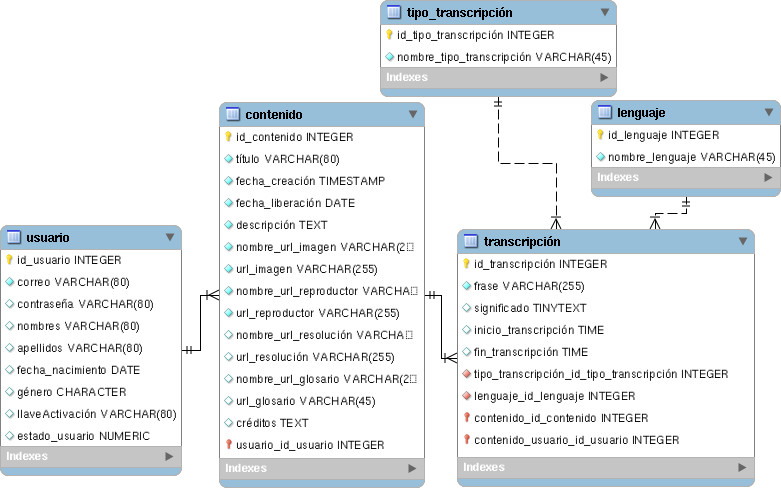
\includegraphics[scale=0.4]{modelTranslation}
	}
	\captionof{figure}{Modelo Transcripci\'{o}n}
	\source{fuente: (Elaboraci\'{o}n Propia)}
	\label{fig:Modelo Transcripci\'{o}n}
\end{minipage}

\subsection{Componente}

En la Figura \ref{fig:Formulario Registro Glosario} se representa la
funcionalidad de creaci\'{o}n de glosario representado en un frase
, lenguaje destino, significado. 

\begin{minipage}{1.0\textwidth}
	\centering
	\fbox{
		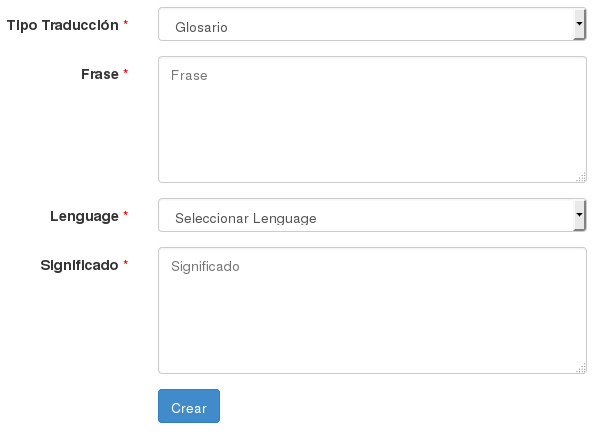
\includegraphics[scale=0.6]{formGlossary}
	}
	\captionof{figure}{Formulario Registro Glosario}
	\source{fuente: (Elaboraci\'{o}n Propia)}
	\label{fig:Formulario Registro Glosario}
\end{minipage}

En la Figura \ref{fig:Diagrama Estados Karaoke} se define la estructura la
que se tom\'{o} en cuenta para la elaboraci\'{o}n del subtitulado de una frase
para definir tanto para el subtitulado origen, subtitulado destino, tiempos 
inicio, tiempo fin de una frase.

\begin{minipage}{1.0\textwidth}
	\centering
	\fbox{
		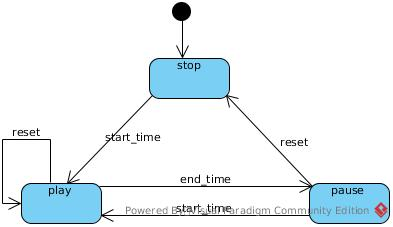
\includegraphics[scale=0.7]{stateLyric}
	}
	\captionof{figure}{Diagrama Estados Karaoke}
	\source{fuente: (Elaboraci\'{o}n Propia)}
	\label{fig:Diagrama Estados Karaoke}
\end{minipage}

En la Figura \ref{fig:Formulario Registro Transcripci\'{o}n} se representa los 
distintos campos necesarios para realizar el subtitulado del lenguaje origen, 
lenguaje destino, tomando en cuenta el reproductor del podcast que es fundamental
para la asignaci\'{o}n.

\begin{minipage}{1.0\textwidth}
	\centering
	\fbox{
		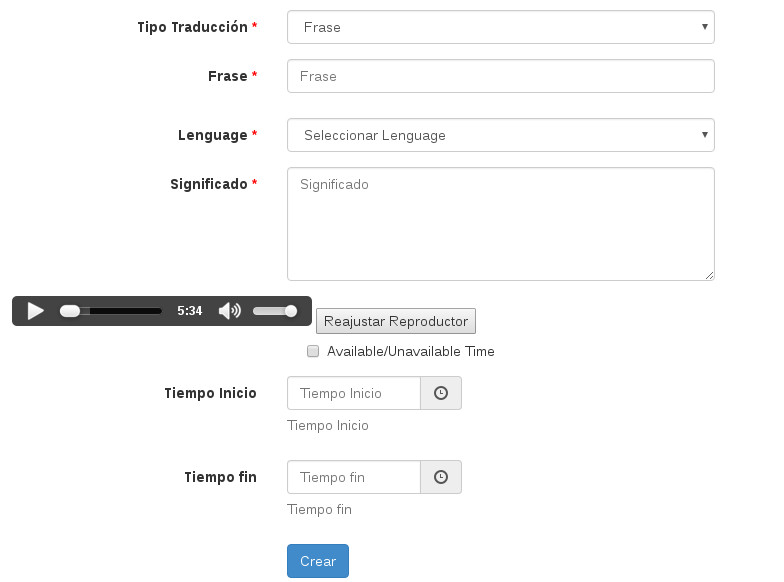
\includegraphics[scale=0.6]{formLyric}
	}
	\captionof{figure}{Formulario Registro Transcripci\'{o}n}
	\source{fuente: (Elaboraci\'{o}n Propia)}
	\label{fig:Formulario Registro Transcripci\'{o}n}
\end{minipage}

\subsection{Implementaci\'{o}n de Componente}

\begin{itemize}

\item \textbf{Implementaci\'{o}n en el Cliente}
Se define la funcionalidad para obtener dos listas en los siguiente: 
Transcripci\'{o}n lenguaje origen propio podcast, Transcripci\'{o}n
a un lenguaje destino para mayor comprension sobre los rol Autorregulado.

\begin{lstlisting}[caption={Llenado elementos subtitulado}, label={lst:fillSubtitle}]
// get object audio player
var myPlayer = document.getElementById("audio-player");
// flag for run one time
var flag = false;
<?php if (isset($model_translation)): ?>
// add event play listener
myPlayer.addEventListener("play", function () {
// verify no change flag
if (!flag) {
// get property through ajax
$.ajax({
type: "POST",
url: "<?php echo CController::createUrl('Translation/getItemSentences'
        ); ?>",
data: {
idTypeTranslation: "<?php echo Yii::app()->params[''
    . 'idTypeTranslationSentence']; ?>",
idContent: "<?php echo Yii::app()->getRequest()->getParam('id_content'
        ); ?>",
idUser: "<?php echo Yii::app()->getRequest()->getParam('user_id_user'
        ); ?>",
idLanguage: "<?php echo $model_translation->language_id_language; ?>"
},
dataType: "html",
success: function (data) {
var div = document.getElementById("idSentence");
div.innerHTML = data;
}
});
.....
// change flag
flag = true;
// call function for show karaoke
play(myPlayer);
}
}, false);
<?php endif; ?>
\end{lstlisting}

\item \textbf{Implementaci\'{o}n en el Cliente}
Se define la siguiente funci\'{o}n, donde se realiza las acciones necesarias para
mostrar/ocultar el subtitulado del lenguage origen sujeto a la acci\'{o}n de un 
bot\'{o}n.  

\begin{lstlisting}[]
function play(myPlayer) {
var controlDuplicate = [];
myPlayer.ontimeupdate = function () {
// get currentTime player
var currentTimePhrase = myPlayer.currentTime;
// identifier for start_translation, end_translation
var currentIDStart = "";
var currentIDEnd = "";
// time converter min:seg
var timeConvert = "";
//convert from seg:miliseg to min:seg
var hr = Math.floor(currentTimePhrase / 3600);
var min = Math.floor((currentTimePhrase - (hr * 3600)) / 60);
var sec = Math.floor(currentTimePhrase - (hr * 3600) - (min * 60));
// if min is less 10 add 0
if (min < 10) {
    min = "0" + min;
}
// if sec is less 10 add 0
if (sec < 10) {
    sec = "0" + sec;
}
timeConvert = min + ':' + sec + ':00';
if (controlDuplicate.length == 0) {
    controlDuplicate.push(timeConvert);
$('#idSentence li').filter(':not([start_time_translation]), \n\
    [start_time_translation="' + timeConvert + '"]').addClass(
    'sentence_show');
...
} else if (controlDuplicate[controlDuplicate.length - 1] != timeConvert) {
    controlDuplicate.push(timeConvert);
$('#idSentence li').filter(':not([start_time_translation]), \n\
    [start_time_translation="'+ timeConvert + '"]').addClass(
    'sentence_show');
$('#idSentence li').filter(':not([start_time_translation]), \n\
    [end_time_translation="' + timeConvert + '"]').removeClass(
    'sentence_show');
...
}
};
}     
\end{lstlisting}

\end{itemize}

\subsection{Problema/Soluci\'{o}n de Componente}

Se considera las siguientes dificultades que surgieron para la implementaci\'{o}n
para Mecanismos de Transcripci\'{o}n.

\begin{itemize}

\item Definici\'{o}n de segundos, minutos para tiempo inicio, tiempo final frase inicial.
\item Definici\'{o}n de campos: tiempo inicio, tiempo final para la frases.

\end{itemize}

\begin{enumerate}
\item \textbf{Definir Tiempos}
La siguiente funcionalidad se debe para realizar el control de la definici\'{o}n
de campos tiempo inicio, tiempo fin en base al reproductor definido para el podcast,
tomando en cuenta restricciones de opciones.
\begin{lstlisting}[]
var myPlayer = document.getElementById("playerMyTranslation");
myPlayer.addEventListener("play", function () {
var status_start_translation = document.getElementById(
    'start_translation').disabled;
if (!status_start_translation) {
var second_start_translation = Math.floor(myPlayer.
    currentTime % 60);
if (second_start_translation < 10) {
    second_start_translation = "0" + 
    second_start_translation;
}
var minute_start_translation = Math.floor((myPlayer.
        currentTime / 60) % 60);
if (minute_start_translation < 10) {
    minute_start_translation = "0" + 
    minute_start_translation;
}
document.getElementById('start_translation').value = 
    minute_start_translation +':' + second_start_translation;
}
}, false);

...
\end{lstlisting}

El manejo de minutos y segundos extraidos de un reproductor se tomen en cuenta
que para segundos y minutos es conveniente agregar un cero si se encuentra como
unidad entera.

\item \textbf{Frase}

La siguiente funcionalidad se debe para realizar el reset de los campos tiempo
inicio, tiempo fin, como del reproductor a un estado inicial.

\begin{lstlisting}[]
function resetPlayer() {
var status_start_translation = document.getElementById(
    'start_translation').disabled;
var status_end_translation = document.getElementById(
    'end_translation').disabled;
var myPlayer = document.getElementById("playerMyTranslation");
if (!status_start_translation && !status_end_translation) {
    if (myPlayer.play) {
    myPlayer.currentTime = 0;
    // set start translation
    document.getElementById('start_translation').value = 0;
    // set end translalation
    document.getElementById('end_translation').value = 0;
    }
}
}
\end{lstlisting}

\end{enumerate}

\section{\textquestiondown C\'{o}mo facilitar representaci\'{o}n de Subtitulado y Glosario?}

Se desea utilizar un mecanismo para poder agregar contenido sem\'{a}ntico a las
siguientes funcionalidades 

\subsection{Componente}

Se facilita el esquema de representaci\'{o}n de un microformato h-entry para la
representaci\'{o}n de un Glosario de podcast. \cite{hEntry}

\textbf{h-entry}

\begin{itemize}

\item \textbf{p-name} nombre entrada/t\'{i}tulo
\item \textbf{p-summary} breve resumen entrada
\item \textbf{e-content} contenido completo entrada
\item \textbf{dt-published} cuando se public\'{o} la entrada
\item \textbf{dt-updated} cuando se actualiza la entrada
\item \textbf{p-author} que escribi\'{o} la entrada, opcionalmente incorporados
h-card
\item \textbf{p-category} categor\'{i}a entrada tags
\item \textbf{u-url} URL del enlace permanente entrada
\item \textbf{u-uid} identificador \'{u}nico universal, la entrada URL can\'{o}nica
normalmente
\item \textbf{p-location} la ubicaci\'{o}n de la entrada fue publicada a partir,
opcionalmente embed h-card, or h-geo
\item \textbf{u-syndication} URL de copias sindicatos de este post, La propiedad
equivalente de rel-syndication
\item \textbf{u-in-reply-to} la URL cual h-entry se considera respuesta a, 
opcionalmente una h-cite

\end{itemize}

En la Figura \ref{fig:Presentaci\'{o}n Glosario} se da a conocer la funcionalidad
de glosario perteneciente a cada podast audio, que tiene los elementos: frase,
descripci\'{o}n.

\begin{minipage}{1.0\textwidth}
	\centering
	\fbox{
		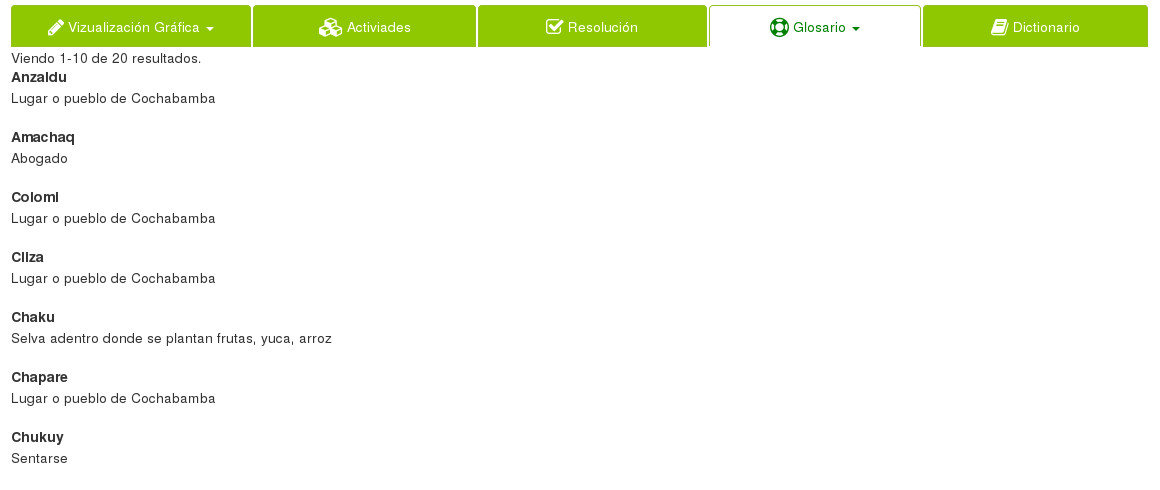
\includegraphics[scale=0.5]{glossary}
	}
	\captionof{figure}{Presentaci\'{o}n Glosario}
	\source{fuente: (Elaboraci\'{o}n Propia)}
	\label{fig:Presentaci\'{o}n Glosario}
\end{minipage}

Se debe agregar contenido sem\'{a}ntico al Subtitulado, entonces se realizo una
extensi\'{o}n a microformatos 2 con el concepto de reutilizaci\'{o}n de 
microformatos base para contrucciones m\'{a}s complejas a continuaci\'{o}n se 
facilita el dise\~{n}o del esquemas. \cite{microformats2}

\textbf{microformats 2}

\begin{itemize}

\item 'h-*' de nombres de clase r\'{a}iz
\item 'p-*' para las caracter\'{i}sticas simples (texto)
\item 'u-*' para las caracter\'{i}sticas URL
\item 'dt-*' para la caracter\'{i}sticas de fecha/hora
\item 'e-*' para las propiedades de marcado incrustado
 
\end{itemize}

Se realiza la siguiente representaci\'{o}n sobre un esquema de tal manera que 
se pueda realizar la sincronizaci\'{o}n del reproductor con subtitulado.

\begin{itemize}

\item \textbf{h-x-lyrics} ra\'{i}z de esquema
\item \textbf{p-lyric h-x-lyric} contenedora de elementos
\item \textbf{p-start-time} representa tiempo inicio
\item \textbf{p-content} representa contenido
\item \textbf{p-end-time} representa tiempo fin

\end{itemize}


En la Figura \ref{fig:Presentaci\'{o}n Subtitulado} se muestra la funcionalidad
de Subtitulado contemplando sincronizaci\'{o}n del reproductor, se muestra dos 
elementos transcripci\'{o}n lenguaje origen, traducci\'{o}n lenguaje destino para. 

\begin{minipage}{1.0\textwidth}
	\centering
	\fbox{
		
\includegraphics[scale=0.6]{lyric}
	}
	\captionof{figure}{Presentaci\'{o}n Substitulado}
	\source{fuente: (Elaboraci\'{o}n Propia)}
	\label{fig:Presentaci\'{o}n Subtitulado}
\end{minipage}

\subsection{Implementaci\'{o}n de Componente}

\begin{itemize}

\item \textbf{Implementaci\'{o}n en el Cliente}
Se define la siguiente agregaci\'{o}n de contenido sem\'{a}ntico para la 
representaci\'{o}n de un glosario tomando en cuenta un microformato base h-entry.

\begin{lstlisting}[language = PHP]
<dl class="h-entry">
    <dt class="p-name">
        <?php echo $data->sentence; ?> 
    </dt> 
    <dd class="p-content">
        <?php echo $data->meaning; ?> 
    </dd>
</dl>
\end{lstlisting}

\item \textbf{Implementaci\'{o}n en el Cliente}
Se define la siguiente agregaci\'{o}n de contenido sem\'{a}ntico de un Subtitulado
brindando que la informaci\'{o}n el mismoque sirve de base.

\begin{lstlisting}[language = PHP]
<div>
<ul class="h-sentence-lyrics ul_hide">
<?php foreach ($model_translations as $translation): ?>  
<li class="p-lyric h-sentence-lyric"> 
<time class="p-start-time"> <?php echo 
    $translation->start_translation; ?> </time>    
<span class="p-content" > <?php echo $translation->sentence
    ; ?></span>
<time class="p-end-time"> <?php echo 
    $translation->end_translation;?> </time>
</li>
<?php endforeach; ?>
</ul>
...
</div>
\end{lstlisting}

\end{itemize}

\subsection{Problema/Soluci\'{o}n de Componente}

Se considera los diferentes dificultades que se tubieron dentro la agregaci\'{o}n
de contenido sem\'{a}ntico sobre la capa vista del sistema.

\begin{itemize}

\item uso de HTML5 \footnote{HTML5: Es una vesi\'{o}n del lenguaje de marcado
de hypertexto, el lenguaje de programaci\'{o}n est\'{a}ndar para describir el
contenido y la apariencia de las p\'{a}ginas Web \cite{html5}}  para agregar 
contenido sem\'{a}ntico
\item agregaci\'{o}n de microformatos lado del Servidor

\end{itemize}

\begin{enumerate}

\item \textbf{Uso de HTML5}

Se debe a que en los sprint: 11, 12, 13 compuesto cada sprint por un tiempo de
15 d\'{i}as h\'{a}viles, se recomienda utilizar documentos HTML5 para evitar
problemas como reconocimiento de microformatos, servicios externos extractores
de informaci\'{o}n.

\item \textbf{Llenado en lenguaje Servidor}

Para realizar el evento de subtitulado inicialmente se penso utilizar la 
funcionalidad Segmento C\'{o}digo \ref{lst:fillSubtitle} que realiza el llenado
de elementos por una sola llamda AJAX \footnote{AJAX: (Asynchronous JavaScript
and XML) is a method of bulding interactive applications for the Web that 
process user request immediately \cite{ajax}} , pero luego se 
considero que al momento de utilizar un servicio extractor externo este no 
funcina correctamente asi que se opto por realizar el llenado en lado del 
servidor.

\begin{lstlisting}[language = PHP]
public function actionViewContent($id_content, $user_id_user, 
    $type_content_id_type_content, $category_id_category) {
Yii::app()->theme = 'front';
//...
// get property kareoke
$model_translations = Translation::model()->findAllByAttributes(
array('type_translation_id_type_translation' => 
$type_content_id_type_content, 'content_id_content' => $id_content,
'content_user_id_user' => $user_id_user), array('order' => 
'start_translation asc'));
//...
// render view
$this->render('viewContent', array('model' => $model, 'model_user'
=> $model_user, 'model_detail_subscriptions' => 
$model_detail_subscriptions, 'model_translate' => $model_translate,
'model_translation' => $model_translation, 'model_translations' => 
$model_translations));
}
\end{lstlisting}

\end{enumerate}

\section{\textquestiondown C\'{o}mo facilitar pruebas de Servicio Agregador de Noticias, Reproducci\'{o}n Audio y Video?}

Para implementar pruebas sobre servicio agregador de noticias se utilizaron pruebas
funcionales contemplando la capa del modelo de datos y para la situaci\'{o}n de pruebas
de reproducci\'{o}n Audio, Video se tubo que tener soporte de emulador web para
automatizar pruebas de integraci\'{o}n estas solo contemplan la capa visa de la
arquitectura del proyecto. 

\subsection{Componente}

En la Figura \ref{fig:Diagrama Clases Dependencia Subscripci\'{o}n} se puede
apreciar el criterio optado para implementar test \footnote{test: Las pruebas
de software es un m\'{e}todo de evaluaci\'{o}n de la funcionalidad de un 
programa de software \cite{test}} 
empezando de arriba hacia abajo, se considero el grado dependencia.

\begin{minipage}{1.0\textwidth}
	\centering
	\fbox{
		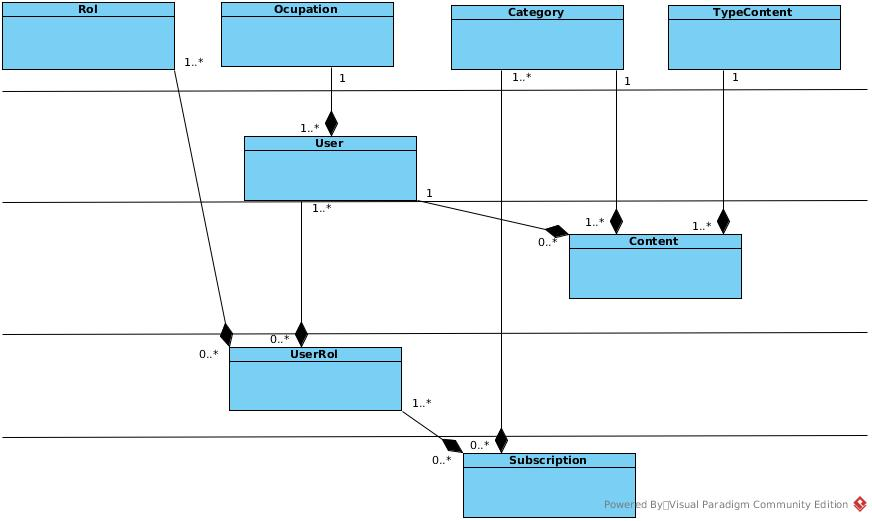
\includegraphics[scale=0.5]{subscriptionTest}
	}
	\captionof{figure}{Diagrama Clases Dependencia Subscripci\'{o}n}
	\source{fuente: (Elaboraci\'{o}n Propia)}
	\label{fig:Diagrama Clases Dependencia Subscripci\'{o}n}
\end{minipage}


\subsection{Reporte Pruebas}

Se define \'{u}nicamente esta secci\'{o}n el uso de Reportes por tratarse de pruebas
funcionales, test integraci\'{o}n.

Los reportes de pruebas se generan en base a la implementaci\'{o}n realizada a
los siguientes m\'{o}dulos que se contenplaron como ser: Subscripci\'{o}n, debido
que el servicio agregador de noticias que se definio en Subsecci\'{o}n \ref{RSS}

% report test 1
\begin{landscape}
\begin{table}
\centering
\begin{tabular}{|l|l|l|l|l|l|}
\hline
\multicolumn{6}{|c|}{\textbf{Test Case Functional}} \\ \hline
\multicolumn{2}{|l|}{Test Case ID:  1} & \multicolumn{2}{l|}{Test Priority: High} & \multicolumn{2}{l|}{Module Name: Category} \\ \hline
\multicolumn{2}{|l|}{Test Title: testCreateUserOneLevelCategory} & \multicolumn{2}{l|}{Test Designed date: 11-02-2016} & \multicolumn{2}{l|}{Test Execution by: 23-05-2016} \\ \hline
\multicolumn{6}{|l|}{Pre-conditions:  BD empty.} \\ \hline
\multicolumn{6}{|l|}{Dependencies:  Category Level zero.} \\ \hline
Test Steps & Test Data & Expected Result & Actual Result & Status & Notes \\ \hline
\begin{tabular}[c]{@{}l@{}}Create category \\ level one\end{tabular} & \begin{tabular}[c]{@{}l@{}}name\_category=QuechuaPsicosocial\\ name\_url\_picture=psicosocial.jpg\\ description\_category=description psicosocial\\ description\_credit=description credit\\ description\_objective=description objective\end{tabular} &  &  & Pass & \begin{tabular}[c]{@{}l@{}}Name category \\ should be\\ unique.\end{tabular} \\ \hline
\end{tabular}
\captionof{table}{Reporte Prueba 1}
\source{fuente: (Elaboraci\'{o}n Propia)}
\label{Reporte Prueba 1}
\end{table}
\end{landscape}

%report test 2
\begin{landscape}
\begin{table}
\centering
\begin{tabular}{|l|l|l|l|l|l|}
\hline
\multicolumn{6}{|c|}{\textbf{Test Case Functional}} \\ \hline
\multicolumn{2}{|l|}{Test Case ID:  2} & \multicolumn{2}{l|}{Test Priority: High} & \multicolumn{2}{l|}{Module Name: Ocupation} \\ \hline
\multicolumn{2}{|l|}{Test Title: testCreateOcupation} & \multicolumn{2}{l|}{Test Designed date: 11-02-2016} & \multicolumn{2}{l|}{Test Execution by: 23-05-2016} \\ \hline
\multicolumn{6}{|l|}{Pre-conditions:  BD empty.} \\ \hline
\multicolumn{6}{|l|}{Dependencies:  Category Level zero.} \\ \hline
Test Steps & Test Data & Expected Result & Actual Result & Status & Notes \\ \hline
\begin{tabular}[c]{@{}l@{}}Create ocupation \\ level one\end{tabular} & name\_ocupation= ocupacion hijo &  &  & Pass & \begin{tabular}[c]{@{}l@{}}Name ocupation\\ should be\\ unique.\end{tabular} \\ \hline
\end{tabular}
\captionof{table}{Reporte Prueba 2}
\source{fuente: (Elaboraci\'{o}n Propia)}
\label{Reporte Prueba 2}
\end{table}
\end{landscape}

% report test 3
\begin{landscape}
\begin{table}
\centering
\begin{tabular}{|l|l|l|l|l|l|}
\hline
\multicolumn{6}{|c|}{\textbf{Test Case Functional}} \\ \hline
\multicolumn{2}{|l|}{Test Case ID:  3} & \multicolumn{2}{l|}{Test Priority: High} & \multicolumn{2}{l|}{Module Name: Rol} \\ \hline
\multicolumn{2}{|l|}{Test Title: testCreateRol} & \multicolumn{2}{l|}{Test Designed date: 12-02-2016} & \multicolumn{2}{l|}{Test Execution by: 23-05-2016} \\ \hline
\multicolumn{6}{|l|}{Pre-conditions:  name\_rol=autorregulado.} \\ \hline
\multicolumn{6}{|l|}{Dependencies:} \\ \hline
Test Steps & Test Data & Expected Result & Actual Result & Status & Notes \\ \hline
\begin{tabular}[c]{@{}l@{}}Create ocupation \\ level one\end{tabular} & name\_rol= autorregulado &  &  & Pass & \begin{tabular}[c]{@{}l@{}}Name rol\\ should be\\ unique.\end{tabular} \\ \hline
\end{tabular}
\captionof{table}{Reporte Prueba 3}
\source{fuente: (Elaboraci\'{o}n Propia)}
\label{Reporte Prueba 3}
\end{table}
\end{landscape}

% report test 4
\begin{landscape}
\begin{table}
\centering
\begin{tabular}{|l|l|l|l|l|l|}
\hline
\multicolumn{6}{|c|}{\textbf{Test Case Functional}} \\ \hline
\multicolumn{2}{|l|}{Test Case ID:  4} & \multicolumn{2}{l|}{Test Priority: High} & \multicolumn{2}{l|}{Module Name: User} \\ \hline
\multicolumn{2}{|l|}{Test Title: testCreateUserOneLevelOcupation} & \multicolumn{2}{l|}{Test Designed date: 18-02-2016} & \multicolumn{2}{l|}{Test Execution by: 23-05-2016} \\ \hline
\multicolumn{6}{|l|}{Pre-conditions:  User available.} \\ \hline
\multicolumn{6}{|l|}{Dependencies:  Ocupation} \\ \hline
Test Steps & Test Data & Expected Result & Actual Result & Status & Notes \\ \hline
\begin{tabular}[c]{@{}l@{}}Create ocupation \\ level one\end{tabular} & \begin{tabular}[c]{@{}l@{}}email=juan@gmail.com\\ username=omarhuanca\\ password=123\\ state\_user=1\\ activationKey=1a2b3c\end{tabular} &  &  & Pass & \begin{tabular}[c]{@{}l@{}}Username, \\ email address\\ should be unique.\end{tabular} \\ \hline
\end{tabular}
\captionof{table}{Reporte Prueba 4}
\source{fuente: (Elaboraci\'{o}n Propia)}
\label{Reporte Prueba 4}
\end{table} 
\end{landscape}

% report test 5
\begin{landscape}
\begin{table}
\centering
\begin{tabular}{|l|l|l|l|l|l|}
\hline
\multicolumn{6}{|c|}{\textbf{Test Case Functional}} \\ \hline
\multicolumn{2}{|l|}{Test Case ID:  5} & \multicolumn{2}{l|}{Test Priority: Medium} & \multicolumn{2}{l|}{Module Name: Content} \\ \hline
\multicolumn{2}{|l|}{Test Title: testCreateContentTypeAudio} & \multicolumn{2}{l|}{Test Designed date: 18-02-2016} & \multicolumn{2}{l|}{Test Execution by: 23-05-2016} \\ \hline
\multicolumn{6}{|l|}{Pre-conditions: User available, Content available.} \\ \hline
\multicolumn{6}{|l|}{Dependencies: User, Ocupation, Category, TypeContent} \\ \hline
Test Steps & Test Data & Expected Result & Actual Result & Status & Notes \\ \hline
Input fields & \begin{tabular}[c]{@{}l@{}}title=Chapter 1\\ date\_create=00-02-2016\\ date\_leave=00-02-2016\\ summary = summary\\ name\_url\_picture=picture chapter 1\\ name\_url\_player=player chapter 1\\ name\_url\_answer=document answer 1\\ credit= credit chapter 1\\ content\_status=1\end{tabular} &  &  & Pass & \begin{tabular}[c]{@{}l@{}}Date leave \\ greater than\\ date create.\end{tabular} \\ \hline
\end{tabular}
\captionof{table}{Reporte Prueba 5}
\source{fuente: (Elaboraci\'{o}n Propia)}
\label{Reporte Prueba 5}
\end{table}
\end{landscape}

% report test 6
\begin{landscape}
\begin{table}
\centering
\begin{tabular}{|l|l|l|l|l|l|}
\hline
\multicolumn{6}{|c|}{\textbf{Test Case Functional}} \\ \hline
\multicolumn{2}{|l|}{Test Case ID:  6} & \multicolumn{2}{l|}{Test Priority: Medium} & \multicolumn{2}{l|}{Module Name: UserRol} \\ \hline
\multicolumn{2}{|l|}{Test Title: testCreateUserRol} & \multicolumn{2}{l|}{Test Designed date: 18-02-2016} & \multicolumn{2}{l|}{Test Execution by: 23-05-2016} \\ \hline
\multicolumn{6}{|l|}{Pre-conditions: User available.} \\ \hline
\multicolumn{6}{|l|}{Dependencies: Rol, User, Ocupation.} \\ \hline
Test Steps & Test Data & Expected Result & Actual Result & Status & Notes \\ \hline
Input fields & \begin{tabular}[c]{@{}l@{}}user\_id\_user = id\_user\\ rol\_id\_rol=id\_rol\end{tabular} &  &  & Pass &  \\ \hline
\end{tabular}
\captionof{table}{Reporte Prueba 6}
\source{fuente: (Elaboraci\'{o}n Propia)}
\label{Reporte Prueba 6}
\end{table}
\end{landscape}

% report test 7
\begin{landscape}
\begin{table}
\centering
\begin{tabular}{|l|l|l|l|l|l|}
\hline
\multicolumn{6}{|c|}{\textbf{Test Case Functional}} \\ \hline
\multicolumn{2}{|l|}{Test Case ID:  7} & \multicolumn{2}{l|}{Test Priority: High} & \multicolumn{2}{l|}{Module Name: Subscription} \\ \hline
\multicolumn{2}{|l|}{Test Title: testCreateSubscription} & \multicolumn{2}{l|}{Test Designed date: 18-02-2016} & \multicolumn{2}{l|}{Test Execution by: 23-05-2016} \\ \hline
\multicolumn{6}{|l|}{Pre-conditions: User available, Content available.} \\ \hline
\multicolumn{6}{|l|}{Dependencies: UserRol, User, Ocupation, Rol, Category} \\ \hline
Test Steps & Test Data & Expected Result & Actual Result & Status & Notes \\ \hline
Input fields & \begin{tabular}[c]{@{}l@{}}category\_id\_category = categoryChild.id\_category\\ id\_user\_rol=userRol.id\_user\_rol\\ user\_id\_user=userRol.user\_id\_user\\ rol\_id\_rol=userRol.rol\_id\_rol\end{tabular} &  &  & Pass &  \\ \hline
\end{tabular}
\captionof{table}{Reporte Prueba 7}
\source{fuente: (Elaboraci\'{o}n Propia)}
\label{Reporte Prueba 7}
\end{table}
\end{landscape}

% report test 8
\begin{landscape}
\begin{table}
\centering
\begin{tabular}{|l|l|l|l|l|l|}
\hline
\multicolumn{6}{|c|}{\textbf{Test Case Integration}} \\ \hline
\multicolumn{2}{|l|}{Test Case ID:  8} & \multicolumn{2}{l|}{Test Priority: Low} & \multicolumn{2}{l|}{Module Name: Content} \\ \hline
\multicolumn{2}{|l|}{Test Title: testPlayAudioLocalHost} & \multicolumn{2}{l|}{Test Designed date: 15-03-2016} & \multicolumn{2}{l|}{Test Execution by: 23-05-2016} \\ \hline
\multicolumn{6}{|l|}{Pre-conditions: Content available, phpunit installed, Selenium webdriver running.} \\ \hline
\multicolumn{6}{|l|}{Dependencies: User, Category, TypeContent.} \\ \hline
Test Steps & Test Data & Expected Result & Actual Result & Status & Notes \\ \hline
Get URL resource & \begin{tabular}[c]{@{}l@{}}http://localhost/plataformaeducativalael/content/\\ viewContent?id\_content=1\&user\_id\_user=27\&\\ type\_content\_id\_type\_content=1\&\\ category\_id\_category=2\end{tabular} &  &  & Pass &  \\ \hline
\end{tabular}
\captionof{table}{Reporte Prueba 8}
\source{fuente: (Elaboraci\'{o}n Propia)}
\label{Reporte Prueba 8}
\end{table}
\end{landscape}

% report test 9
\begin{landscape}
\begin{table}
\centering
\begin{tabular}{|l|l|l|l|l|l|}
\hline
\multicolumn{6}{|c|}{\textbf{Test Case Integration}} \\ \hline
\multicolumn{2}{|l|}{Test Case ID:  9} & \multicolumn{2}{l|}{Test Priority: Low} & \multicolumn{2}{l|}{Module Name: Content} \\ \hline
\multicolumn{2}{|l|}{Test Title: testPlayVideoLocalHost} & \multicolumn{2}{l|}{Test Designed date: 15-03-2016} & \multicolumn{2}{l|}{Test Execution by: 23-05-2016} \\ \hline
\multicolumn{6}{|l|}{Pre-conditions: Content available, phpunit installed, Selenium webdriver running.} \\ \hline
\multicolumn{6}{|l|}{Dependencies: User, Category, TypeContent.} \\ \hline
Test Steps & Test Data & Expected Result & Actual Result & Status & Notes \\ \hline
Get URL resource & \begin{tabular}[c]{@{}l@{}}http://localhost/plataformaeducativalael/content/\\ viewContent?id\_content=2\&user\_id\_user=27\&\\ type\_content\_id\_type\_content=2\&\\ category\_id\_category=3\end{tabular} &  &  & Pass &  \\ \hline
\end{tabular}
\captionof{table}{Reporte Prueba 9}
\source{fuente: (Elaboraci\'{o}n Propia)}
\label{Reporte Prueba 9}
\end{table}
\end{landscape}

En la Figura \ref{fig:Ejecuci\'{o}n Test Subscripci\'{o}n} se puede apreciar la
ejecuci\'{o}n del test referente creaci\'{o}n de una subscripci\'{o}n de un 
usuario dirijido a una categor\'{i}a hijo.

\begin{minipage}{1.0\textwidth}
	\centering
	\fbox{
		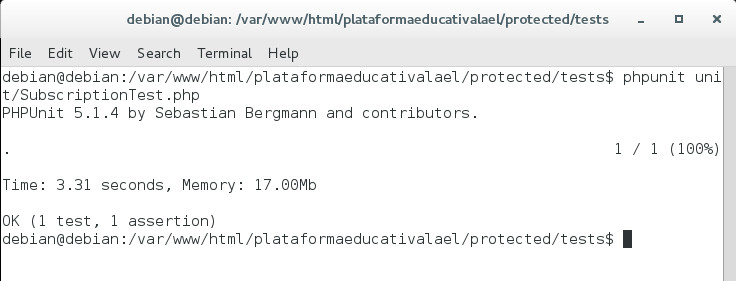
\includegraphics[scale=0.7]{runSubscriptionTest}
	}
	\captionof{figure}{Ejecuci\'{o}n Test Subscripci\'{o}n}
	\source{fuente: (Elaboraci\'{o}n Propia)}
	\label{fig:Ejecuci\'{o}n Test Subscripci\'{o}n}
\end{minipage}


\subsection{Implementaci\'{o}n de Componente}

\begin{itemize}

\item \textbf{Implementaci\'{o}n en el Servidor}
Se define la implementaci\'{o}n de prueba crear subscripci\'{o}n que se describe
el reporte en Cuadro \ref{Reporte Prueba 7}, agregando el grado dependencia
expuesto en la Figura \ref{fig:Diagrama Clases Dependencia Subscripci\'{o}n}

\begin{lstlisting}[language = PHP]
// before each run test
public function setUp() {
    parent::setUp();
    ...
}
// after each run test
public function tearDown() {
    parent::tearDown();
    ...
}
public function testCreateSubscription() {
    // create subscription
    $subscription = new Subscription();
    $subscription->setAttributes(array(
    'category_id_category' => $this->categoryChild->id_category,
    'id_user_rol' => $this->userRol->id_user_rol,
    'user_id_user' => $this->userRol->user_id_user,
    'rol_id_rol' => $this->userRol->rol_id_rol
    ), false);
    $this->assertTrue($subscription->save(false));
}
\end{lstlisting}

\item \textbf{Implementaci\'{o}n en el Servidor}
Se define la funcionalidad de control a nivel de la capa modelo de Arquitectura
de proyecto para realizar control, manejo haciendo uso de una transaccion. 
\footnote{transaccion: Una secuencia de intercambio de informaci\'{o}n y el 
trabajo relacionado que se trata como una unidad a efectos de satisfacer una
solicitud como para asegurar la integridad de la base de datos \cite{transaction}} 

\begin{lstlisting}[language = PHP]
public function beforeSave() {
$res = false;
if ($this->isNewRecord) {
// start transaction
$transaction = $this->dbConnection->beginTransaction();
...
$category = Category::model()->findByPk(array('id_category' => 
    $this->category_id_category));
if (isset($category)) {
    if ($category->category_id_category != null) {
    $content = Content::model()->findByAttributes(array(
    'category_id_category' => $category->id_category, 
    'content_status' => Yii::app()->params['stateContentAvailable']));
    if (isset($content)) {
    $user = User::model()->findByAttributes(array('id_user' => 
        $content->user_id_user, 'state_user' => 
        Yii::app()->params['stateUserAvailable']));
        if (isset($user)) {
        $res = true;
        }
    }
    }
}
if ($res) {
    $transaction->commit();
} else {
        $transaction->rollback();
}
...
} else {
    $res = true;
}
    return $res;
}
\end{lstlisting}

\end{itemize}

\subsection{Problema/Soluci\'{o}n de Componente}

Se consideran las siguientes dificultades que surgieron:

\begin{itemize}

\item Instalar PHPUnit y dependencias desde composer
\item Verificar funcionalidad de Firefox sobre consola
\item Configurar archivos bootstrap y phpunit.xml sobre Yii
\item Editar archivos CWebTestCase para reconocimiento de comandos phpunit

\end{itemize}

\begin{enumerate}

\item \textbf{PHPUnit, Dependencias}
Se recomienda realizar la instalaci\'{o}n de phpunit por medio de composer 
\footnote{composer: Es un gestor de dependencias para PHP. Composer 
gestionar\'{a} las dependencias que se requieren en un proyecto por ejemplo 
\cite{composer}} para agregar contenido dependencias dentro la carpeta  
/project/protected/composer.json y empezar utilizar sentencias para implementar
test.

\begin{lstlisting}[]
{
    "name": "kevin/protected",
    "authors": [
        {
            "name": "kevin",
            "email": "kevinflorenzdaus@gmail.com"
        }
    ],
    "require-dev": {
        "phpunit/phpunit": "3.7.*",
        "phpunit/phpunit-selenium": ">=1.2",
        "phpunit/dbunit": ">=1.2",
        "phpunit/phpunit-story": "*"
    }
}
\end{lstlisting}

\item \textbf{Firefox sobre Consola}
Particularmente se desarrollo el proyecto sobre una distribuci\'{o}n Debian 8,
para el mismo viene con un navegador denominado iceweasel, se tubo que realizar
iceweasel por mozilla firefox.

\begin{lstlisting}[]
$ wget ftp://ftp.mozilla.org/pub/mozilla.org/firefox/
	releases/Y.0/linux-x86_64/en-US/firefox-Y.0.tar.bz2
cd /home/hugh/
$ tar -xjvf firefox-Y.0.tar.bz2
$ sudo rm -rf /opt/firefox*
$ sudo mv firefox /opt/firefoxY.0
$ sudo ln -sf /opt/firefoxY.0/firefox /usr/bin/firefox
\end{lstlisting}

Se tubo problemas en el momento de ejecutar firefox sobre selenium web driver
para contemplar pruebas de integraci\'{o}n, asi que lo recomendable es realizar
la instalaci\'{o}n de navegador de forma manual.

\item \textbf{Configurar Archivos bootstrap y phpunit}
Este archivo es tan especial porque es como el gui\'{o}n de entrada y es el punto
de partida cuando se ejecuta una serie de pruebas. \cite{testing}

\begin{lstlisting}[language=PHP]
// change the following paths if necessary
$vendors=dirname(__FILE__).'/../vendor/autoload.php';
$yiit=dirname(__FILE__).'/../../framework/yiit.php';
$config=dirname(__FILE__).'/../config/test.php';
// required file
require_once($vendors);
require_once($yiit);
require_once(dirname(__FILE__).'/WebTestCase.php');
// config app
Yii::createWebApplication($config);
\end{lstlisting}

El archivo phpunit.xml es aquel archivo de configuraci\'{o}n, tambi\'{e}n se 
define el navegador a ejecutarse en pruebas de integraci\'{o}n haciendo uso
de selenium web driver.

\begin{lstlisting}[]
<phpunit bootstrap="bootstrap.php"
	colors="false"
    convertErrorsToExceptions="true"
    convertNoticesToExceptions="true"
    convertWarningsToExceptions="true"
  	stopOnFailure="false">
<selenium>
	<browser name="Google Chrome" browser="*chrome" />
    <browser name="Firefox" browser="*firefox" />
</selenium>
</phpunit>
\end{lstlisting}

\item \textbf{Editar Archivo CWebTestCase}
Se tiene el la siguiente configuraci\'{o}n por defecto, la cual se encuentra en
el archivo /project/framework/test/CWebTestCase.php

\begin{lstlisting}[language=PHP, caption={Cabecera Archivo CWebTestCase}, label={lst:fileCWebTestCase}]
<?php
/**
 * This file contains the CWebTestCase class.
 *
 * @author Qiang Xue <qiang.xue@gmail.com>
 * @link http://www.yiiframework.com/
 * @copyright 2008-2013 Yii Software LLC
 * @license http://www.yiiframework.com/license/
 */
Yii::import('system.test.CTestCase');
require_once('PHPUnit/Extensions/SeleniumTestCase.php');
\end{lstlisting}

Para poder tener acceso a la API \footnote{API: Es una interfaz a trav\'{e}s 
del cual se accede a otra persona o c\'{o}digo a trav\'{e}s del cual el 
c\'{o}digo de otra persona accede a la suya. En efecto los m\'{e}todos 
p\'{u}plicos y propiedades \cite{api}} de implementaci\'{o}n de test sobre Yii
1.x es conveniente reemplazar en el Segmento C\'{o}digo 
\ref{lst:fileCWebTestCase} en la linea 11 por la instrucci\'{o}n definida en la
linea 1 del Segmento C\'{o}digo \ref{lst:replaceCWebTestCase}

\begin{lstlisting}[language=PHP, caption={Instrucci\'{o}n a Reemplazar}, label={lst:replaceCWebTestCase}]
require_once('../../protected/vendor/phpunit/phpunit-selenium/
	PHPUnit/Extensions/SeleniumTestCase.php');
\end{lstlisting}

\end{enumerate}

\section{Duraci\'{o}n Proyecto}

Se implemento un tiempo de 15 d\'{i}as h\'{a}biles para poder definir un sprint y
el mismo sirvio de pase para poder realizar la estimaci\'{o}n del equipo de 
trabajo con lo que se logro obtener 21 sprints los cuales contemplan: 
implementaci\'{o}n y refactorizaci\'{o}n de funcionalidad.